\documentclass[a4paper,10pt]{article}
\usepackage[top=0.75in, bottom=0.75in, left=0.55in, right=0.85in]{geometry}
\usepackage{graphicx}
\usepackage[latin1]{inputenc}
\usepackage{amsmath}
\usepackage{amsfonts}
\usepackage{amssymb}

\begin{document}

\begin{flushright}
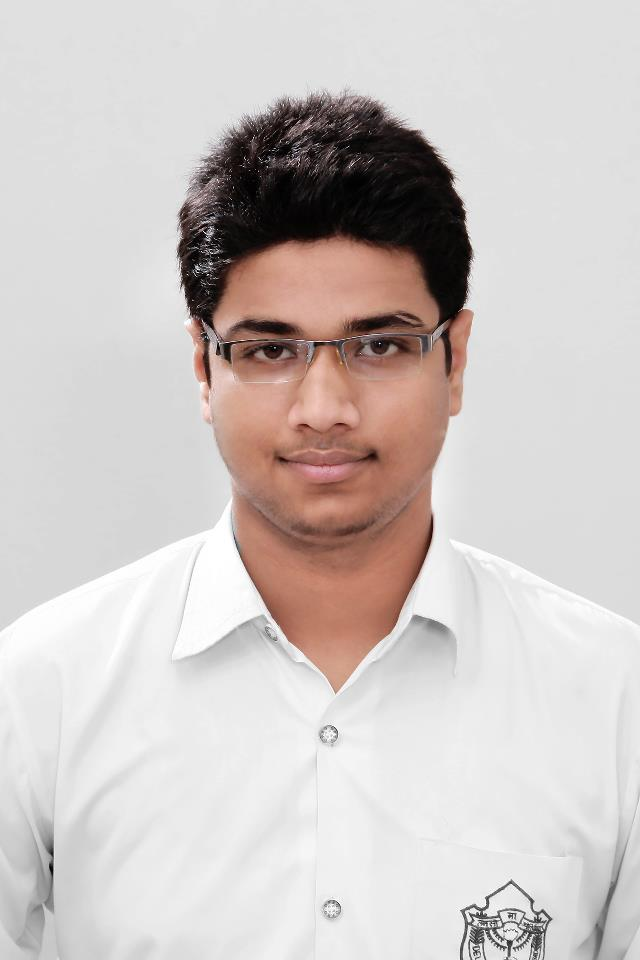
\includegraphics[width=3cm, height=4cm]{dev.jpg}\\
\large
\textbf{\bigskip Divyansh Lohia}
\end{flushright}


\begin{flushleft}
	%contact information
	\textbf{\large Contact Information}:\\
	\hrule
	\bigskip
	\textbf{Address:}            Kd/Ch2 Kavinagar Ghaziabad U.P 201002\\
	\textbf{Contact:}   \texttt{9711794846}\\
	\textbf{Email:}             divyanshlohia95@gmail.com\\ 
	\bigskip
	%career objectives
    \textbf{\large Career Objective:}\\
    \hrule
    \smallskip
    Organize and operate a business venture and assume much of the associated risk and contribute in Make 	In India Project\\
    %education
	\bigskip
	\textbf{\large  Education}:\\
	\hrule
	\bigskip
	\begin{tabular}{|c|c|c|c|c|}
   		\hline \textbf{ Degree}  & \textbf{College/school}  & \textbf{University} & \textbf{Passing Year} 			& 		\textbf{ Pass percentage} \\ 
   		\hline B.Tech Electronics & Maharaja Agrasen College  & Delhi University & 2017 & - \\ 
   		\hline 
			10+2 & Delhi Public School Ghaziabad & - & 2013 & 88 \\
    	\hline
    		10 & Delhi Public School Ghaziabad & - & 2011 & 10 CGPA \\
    		\hline
	\end{tabular}
	%projects
    \textbf{\large Projects:}\\
    \hrule
      \begin{enumerate}
      	\item  Development of Android applications for university
      	\item  Hand gesture controlled robot using xbee
      	\item  Mineit Bot(prototype for detection of mines in form of boxes)
      	\item  Helio Bot(prototype for capturing of solar energy efficiently by movement of solar pannel)
      \end{enumerate}
\end{flushleft}
\end{document}